\documentclass[aspectratio=169]{beamer}

% --- THEME SETUP ---
\usetheme{Madrid}
% \usecolortheme{beaver} % Red/Grey theme for "Top Secret" vibe
\setbeamertemplate{navigation symbols}{} % Hide navigation commands (icons)

% --- CUSTOM WHITE BANNER LOGO SETUP ---
\setbeamercolor{frametitle}{bg=white, fg=blue!70!black}
\setbeamertemplate{frametitle}{%
    \vspace{0.2cm}
    \begin{beamercolorbox}[wd=\paperwidth, ht=0.7cm, dp=0.2cm]{frametitle}
        \hspace*{0.5cm}\usebeamerfont{frametitle}\insertframetitle\hfill
        \raisebox{-0.3cm}{\includegraphics[height=1cm]{logo_univ_bdx.png}}\hspace*{0.5cm}
    \end{beamercolorbox}%
    \begin{tikzpicture}[remember picture,overlay]
        \draw[blue!70!black, thick] (current page.north west) ++(0,-1.3cm) -- ++(\paperwidth,0);
    \end{tikzpicture}
}

% --- PACKAGES ---
\usepackage[utf8]{inputenc}     
\usepackage[T1]{fontenc}
\usepackage{booktabs}
\usepackage{amsmath, amssymb}
\usepackage{tikz}
\usetikzlibrary{shapes.geometric, arrows.meta, positioning, calc}
\usepackage{pgfpages} % For speaker notes

% --- SPEAKER NOTES CONFIG ---
% Enable dual screen: Slides on Left, Notes on Right
\setbeameroption{show notes on second screen=right}
\setbeamertemplate{note page}[plain]

% --- LOGO CONFIG (MOVED TO FRAMETITLE) ---

% --- METADATA ---
\title{Operation Rubicon}
\subtitle{Analyse Cryptographique de la Vulnérabilité Minerva}
\author{Arnaud Gomes}
\institute{Université de Bordeaux}
\date{\today}

\begin{document}

% ==============================================================================
% 1. TITLE
% ==============================================================================
\begin{frame}
    \titlepage
    \note{
        Bonjour à tous. Aujourd'hui je vais vous parler de l'une des plus grandes affaires d'espionnage du 20ème siècle : l'Opération Rubicon.
        
        Pendant près de 50 ans, les agences de renseignement américaine (CIA) et ouest-allemande (BND) ont secrètement possédé la société suisse Crypto AG, qui était alors le leader mondial incontesté de la vente d'équipements de chiffrement et de sécurité des télécommunications pour les diplomates et tous les gouvernements.
        
        L'histoire que je vais vous raconter aujourd'hui montre que la vulnérabilité technique au sein de ces machines n'était pas une simple erreur de code. C'était une véritable porte dérobée (backdoor) mathématique, créée dès le départ pour écouter les communications du monde entier.
    }
\end{frame}

% ==============================================================================
% 2. CONTEXT (MULTIPLE SLIDES)
% ==============================================================================
\section{Contexte Géopolitique}

\begin{frame}{Le Contexte : Le Partenariat CIA / BND}
    \begin{columns}
        \column{0.4\textwidth}
        \textbf{L'Opération Rubicon (Thesaurus)}\\
        \vspace{0.3cm}
        \begin{itemize}
            \item Accord secret signé en 1970.
            \item Achat de Crypto AG via des sociétés écrans au Liechtenstein.
            \item Partage à 50/50 des bénéfices... et des interceptions diplomatiques.
        \end{itemize}

        \column{0.6\textwidth}
        \begin{center}
            \resizebox{\linewidth}{!}{
            \begin{tikzpicture}
                \node[draw=black, fill=red!10, text width=2.8cm, align=center, rounded corners] (cia) at (0,2.5) {
                    \includegraphics[height=1cm]{images/cia_seal.png}\\
                    \vspace{0.1cm}
                    \textbf{NSA / CIA}
                };
                \node[draw=black, fill=gray!20, text width=2.8cm, align=center, rounded corners] (bnd) at (0,-2.5) {
                    \includegraphics[height=1cm]{images/bnd_hq.jpg}\\
                    \vspace{0.1cm}
                    \textbf{ZFA / BND}
                };
                \node[draw=black, fill=blue!10, text width=3.2cm, align=center, rounded corners] (cag) at (6.5,0) {
                    \includegraphics[height=1cm]{images/crypto_ag_logo.png}\\
                    \vspace{0.1cm}
                    \textbf{Crypto AG} \\ 
                    \textit{Zoug, Suisse}
                };

                \draw[-{Latex[length=3mm]}, thick] (cia) to[out=0, in=120] node[above, sloped, midway, font=\footnotesize] {Cahier des charges} (cag);
                \draw[-{Latex[length=3mm]}, thick] (bnd) to[out=0, in=240] node[below, sloped, midway, font=\footnotesize] {Ingénierie} (cag);
                \draw[{Latex[length=3mm]}-, dashed, thick, red] (cia) to[out=-20, in=160] node[below, sloped, midway, font=\footnotesize] {Renseignements} (cag);
            \end{tikzpicture}
            }
        \end{center}
    \end{columns}

    \note{
        Pour bien comprendre la portée de cette attaque, je vais d'abord planter le décor. Tout commence en 1970, en pleine Guerre Froide. La CIA américaine et le BND d'Allemagne de l'Ouest signent un accord secret, nom de code Thesaurus, baptisé par la suite Rubicon.
        
        Ils rachètent secrètement la société Crypto AG, basée à Zoug en Suisse, en utilisant un montage financier très complexe de sociétés écrans. 
        
        L'objectif de cette entité est double : d'une part les deux agences se partagent les énormes bénéfices commerciaux, environ 50/50. Mais surtout, je tenais à insister, la NSA et la ZFA (l'agence ouest-allemande) imposent désormais les algorithmes de chiffrement qui seront implantés dans les machines. Ils contrôlent la chaîne de production.
    }
\end{frame}

\begin{frame}{Le Contexte : "Trusted" Hardware}
    \begin{columns}
        \column{0.5\textwidth}
        \begin{alertblock}{Le Couvert de la Neutralité Suisse}
            Leader mondial du chiffrement matériel (ex: HC-520, HC-570).
            Vendu à +120 pays sous couvert de stricte neutralité.
        \end{alertblock}

        \vspace{0.2cm}
        \textbf{Le Mécanisme Commercial :}
        \begin{itemize}
            \item \textbf{Machines Dédiées :} Boîtiers électromécaniques lourds.
            \item \textbf{Boîte Noire :} Algorithmes propriétaires hardware non-documentés ("Security by Obscurity").
            \item \textbf{Légitimité :} Promesse de sécurité mathématique par Boris Hagelin.
        \end{itemize}

        \column{0.5\textwidth}
        \begin{center}
            \includegraphics[height=3.5cm]{images/hagelin.jpg}\\
            \vspace{0.1cm}
            \tiny \textit{Une machine de type Hagelin CX-52.}
        \end{center}
    \end{columns}

    \note{
        Pourquoi le monde entier a-t-il acheté ces machines ? D'abord, à cause de la Suisse. Crypto AG bénéficiait de l'aura de neutralité politique, ce qui en faisait le fournisseur idéal.
        
        Ensuite, le produit était matériel ("hardware"). Comme vous le voyez ici à droite avec les machines inventées par Boris Hagelin, il s'agissait de blocs lourds, considérés inviolables physiquement.
        Les algorithmes de la série Cryptomatic (HC-500) étaient gravés dans le silicium : aucune spécification ou documentation mathématique n'était fournie. C'est le principe même de la "Security by Obscurity", un concept très dangereux en cryptographie.
    }
\end{frame}

\begin{frame}{Le Contexte : Les Deux Versions (A et B)}
    \begin{columns}
        \column{0.5\textwidth}
        \textbf{Version A : "Alliés"}
        \begin{itemize}
            \item États-Unis, Royaume-Uni, OTAN.
            \item Machines totalement sécurisées.
            \item Algorithme robuste non-compromis.
        \end{itemize}

        \column{0.5\textwidth}
        \textbf{Version B : "Le Reste du Monde"}
        \begin{itemize}
            \item Iran, Libye, Argentine, Inde, Vatican...
            \item Machines comportant la faille \textit{Minerva}.
            \item Messages lisibles en temps réel par NSA/BND.
        \end{itemize}
    \end{columns}
    
    \vspace{0.8cm}
    \begin{center}
        \textit{Même les ingénieurs et commerciaux de Crypto AG (ex: Hans Bühler en Iran) ignoraient manipuler des versions truquées.}
    \end{center}

    \note{
        Ce que les pays clients ignoraient évidemment, c'est que l'usine de Zoug produisait deux versions de la même machine en modifiant juste l'algorithme interne.
        
        La Version A, sécurisée organiquement, était vendue aux pays alliés de l'OTAN, comme le Royaume-Uni ou les Etats-Unis.
        La Version B était destinée au reste du monde : l'Iran, la Libye de Kadhafi, l'Argentine de la junte militaire, l'Inde... Ces machines contenaient la faille Minerva, permettant aux espions de lire les câbles diplomatiques en clair ou presque.
        
        J'ai trouvé fascinant de voir que le degré de secret était tel que même les ingénieurs concepteurs de chez Crypto AG ignoraient qu'ils vendaient des boîtes truquées. Seule une micro-cellule d'ingénieurs mathématiciens concevait la faille pour la NSA !
    }
\end{frame}

% ==============================================================================
% 2.5 HISTORICAL IMPACT SLIDES
% ==============================================================================

\begin{frame}{L'Impact Historique : Exploitation des failles}
    \textbf{Cas n°1 : La Guerre des Malouines (1982)}

    \vspace{0.3cm}
    \begin{itemize}
        \item \textbf{Le Contexte :} Conflit armé entre le Royaume-Uni (Fournisseur "Version A") et l'Argentine (Client Crypto AG "Version B").
        \item \textbf{L'Exploitation :} La junte militaire argentine chiffrait l'intégralité de ses communications navales tactiques avec des machines de la série Hagelin CX-52 / HC-500.
        \item \textbf{Résultat Opérationnel :} La NSA déchiffre les positions navales argentines en temps réel et transmet l'ordre de bataille exact à Londres.
    \end{itemize}

    \vspace{0.5cm}
    \begin{columns}
        \column{0.8\textwidth}
        \begin{alertblock}{La trahison diplomatique parfaite}
            L'Argentine, pensant son canal diplomatique sécurisé, négociait publiquement aux Nations-Unies tout en planifiant des frappes. Margaret Thatcher lisait les télégrammes avant même le président argentin.
        \end{alertblock}
    \end{columns}

    \note{
        Pour bien comprendre comment ce niveau d'espionnage mathématique se traduit sur le terrain, je propose deux exemples historiques majeurs. D'abord, la Guerre des Malouines en 1982.
        
        Lorsque l'Argentine envahit les îles, elle était totalement confiante dans ses communications chiffrées par ses machines Hagelin qu'elle jugeait ultra-modernes. L'erreur fut fatale. Le Royaume-Uni, pays ami des États-Unis et faisant partie de l'OTAN (donc utilisateur de la machine pure Version A), bénéficiait des écoutes totales.
        
        Grâce à la faille Minerva, la NSA craquait en temps réel les communications navales et diplomatiques argentines. Elle transmettait la position des sous-marins et des frégates au commandement de Margaret Thatcher. Dans le monde des agences, on raconte que Londres lisait les plans de la junte militaire plus rapidement que les propres généraux argentins.
    }
\end{frame}

\begin{frame}{L'Impact Historique : L'Iran et la Libye}
    \textbf{Cas n°2 : Espionnage étatique et Anti-terrorisme (Années 70-80)}

    \vspace{0.3cm}
    \begin{columns}
        \column{0.5\textwidth}
        \textbf{Crise des otages en Iran (1979)}
        \begin{itemize}
            \item Crise diplomatique : 52 américains retenus à Téhéran.
            \item Jimmy Carter (USA) observe la diplomatie ennemie en temps réel via l'interception des HC-500 iraniennes.
        \end{itemize}

        \column{0.5\textwidth}
        \textbf{Attentat "La Belle" Berlin (1986)}
        \begin{itemize}
            \item Ronald Reagan accuse Mouammar Kadhafi de l'attentat de Berlin-Ouest.
            \item Preuve formelle : Les télégrammes de "félicitations" libyens chiffrés par Crypto AG explosent silencieusement dans les serveurs de la NSA.
        \end{itemize}
    \end{columns}

    \vspace{0.6cm}
    \textit{Conséquence globale : Durant toute la Guerre Froide, la CIA a écouté plus de 120 pays sans la moindre résistance topologique.}

    \note{
        Je voudrais également aborder le Moyen-Orient. Lors de la Révolution Iranienne de 1979 et de la crise des otages, le régime islamiste utilise massivement les HC-500 "Version B" léguées par le Shah d'Iran. Le président américain Jimmy Carter déchiffre jour par jour les discussions internes du gouvernement de l'Ayatollah Khomeini... alors même que ceux-ci négocient contre lui !
        
        Plus tard, en 1986, lors de la bombe posée dans la discothèque berlinoise "La Belle", le président Ronald Reagan ordonne le bombardement de la Libye. Pour justifier cette frappe, l'administration américaine évoque des "preuves absolues". Ces preuves irréfutables s'avèrent être les câbles libyens chiffrés (des "Félicitations pour Berlin" envoyées de Tripoli) déchiffrés en quelques secondes par la NSA grâce, une fois de plus, à la faille intentionnelle de leurs machines suisses.
        
        Pendant un demi-siècle, ce fut tout l'échiquier mondial de la Guerre Froide qui tombait, de manière transparente.
    }
\end{frame}

% ==============================================================================
% 3. TECHNICAL ARCHITECTURE 
% ==============================================================================
\section{Architecture Technique}

\begin{frame}{Architecture : Chiffrement par Flot}
    \textbf{Modèle Mathématique (Cours Chap. II)}

    \vspace{0.3cm}
    Le système est un \textbf{chiffrement par flot synchrone}.
    Le message clair $m_t$ est chiffré bit à bit avec un flux pseudo-aléatoire $z_t$ (keystream) :
    
    \begin{block}{Équation Fondamentale}
    $$c_t = m_t \oplus z_t$$
    \end{block}

    \vspace{0.3cm}
    \textbf{Avantages dans le Contexte Matériel ($1970-1980$)} :
    \begin{itemize}
        \item Implémentation hardware très économique en portes logiques.
        \item Le déchiffrement est identique au chiffrement ($m_t = c_t \oplus z_t$).
        \item Pas de propagation d'erreur sur la ligne radio/télex.
    \end{itemize}

    \note{
        Je vais maintenant plonger sous le capot technique pour analyser mathématiquement comment la faille a été introduite, en m'appuyant rigoureusement sur le modèle du chapitre II du cours de cryptologie.
        
        Les machines de Crypto AG utilisaient un modèle de "chiffrement par flot synchrone". C'est un principe très calculatoire : le texte clair $m_t$ est chiffré bit par bit par une simple opération d'Ou-Exclusif (XOR) avec un bit de la suite chiffrante $z_t$. 
        
        Pourquoi ont-ils choisi cela dans les années 70-80 ? Pour l'implémentation physique en silicium, que je vais vous montrer. Implémenter un chiffrement par flot en hardware coûte infiniment moins cher en espace et en énergie. De plus, sur des lignes télex imparfaites, la corruption d'un bit de cryptogramme en cas de coupure radio ne corrompt qu'un seul bit de texte décrypté : c'est très résilient !
    }
\end{frame}

\begin{frame}{Le Générateur : Registres à Décalage (LFSR)}
    La sécurité repose sur la suite chiffrante, générée généralement par un ou plusieurs \textbf{LFSR (Linear Feedback Shift Register)}.

    \vspace{0.3cm}
    \begin{center}
    \resizebox{0.9\linewidth}{!}{
    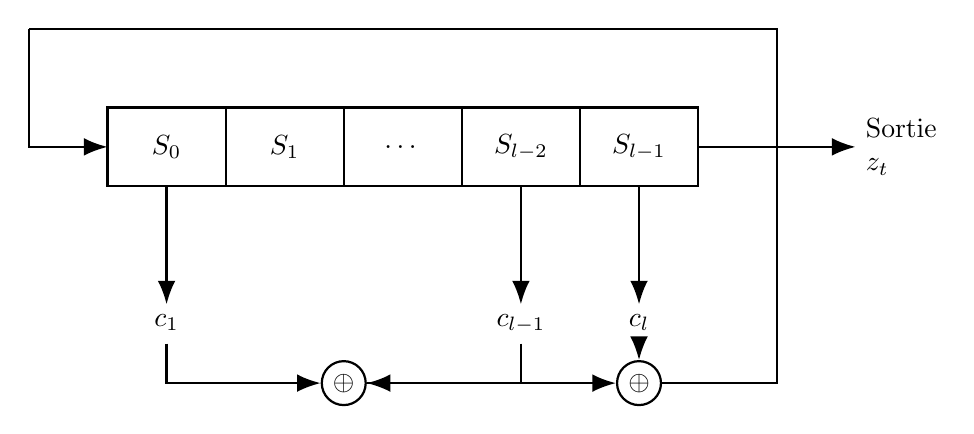
\begin{tikzpicture}[thick]
        % LFSR Boxes
        \draw (0,0) rectangle (1.5,1) node[pos=.5] {$S_{0}$};
        \draw (1.5,0) rectangle (3,1) node[pos=.5] {$S_{1}$};
        \draw (3,0) rectangle (4.5,1) node[pos=.5] {$\dots$};
        \draw (4.5,0) rectangle (6,1) node[pos=.5] {$S_{l-2}$};
        \draw (6,0) rectangle (7.5,1) node[pos=.5] {$S_{l-1}$};
        
        % Taps
        \draw[-{Latex[length=3mm]}] (0.75,0) -- (0.75,-1.5) node[below] {$c_1$};
        \draw[-{Latex[length=3mm]}] (5.25,0) -- (5.25,-1.5) node[below] {$c_{l-1}$};
        \draw[-{Latex[length=3mm]}] (6.75,0) -- (6.75,-1.5) node[below] {$c_l$};
        
        % XOR operations horizontally
        \node[draw, circle, inner sep=2pt] (x1) at (3,-2.5) {$\oplus$};
        \draw[-{Latex[length=3mm]}] (0.75,-2.0) |- (x1);
        \draw[-{Latex[length=3mm]}] (5.25,-2.0) |- (x1);
        
        \node[draw, circle, inner sep=2pt] (x2) at (6.75,-2.5) {$\oplus$};
        \draw[-{Latex[length=3mm]}] (x1) -- (x2);
        \draw[-{Latex[length=3mm]}] (6.75,-2.0) -- (x2);
        
        % Feedback loop
        \draw[-] (x2) -- (8.5,-2.5) -- (8.5,2) -- (-1,2);
        \draw[-{Latex[length=3mm]}] (-1,2) |- (-1,0.5) -- (0,0.5);
        
        % Output
        \draw[-{Latex[length=3mm]}] (7.5,0.5) -- (9.5,0.5) node[right, align=left] {Sortie \\ $z_t$};
    \end{tikzpicture}
    }
    \end{center}

    \vspace{0.2cm}
    \begin{itemize}
        \item État interne au temps $t$ : $S^{(t)} = (S_0^{(t)}, \dots, S_{l-1}^{(t)}) \in \mathbb{F}_2^l$.
        \item Polynôme de rétroaction primitif : $f(X) = 1 \oplus c_1 X \oplus \dots \oplus c_l X^l$
        \item Longueur maximale de la séquence générée avant répétition : $T = 2^l - 1$ (m-suite).
    \end{itemize}

    \note{
        Comme nous l'avons abordé en cours, toute la solidité repose sur le générateur pseudo-aléatoire (le LFSR).
        
        Comme j'ai essayé de l'illustrer sur ce schéma TikZ pour la modélisation matérielle, un registre va conserver en mémoire L bits. A chaque cycle d'horloge, l'appareil décale tous les bits d'une position. Le nouveau bit d'entrée est calculé par la somme modulo 2 des sous-registres.
        L'état va évoluer selon un système d'équations logiques linéaires sur le corps fini $F_2$, et la dynamique du registre est décrite par "le polynôme de rétroaction".
        
        Dans les machines Crypto AG, ces polynômes sont primitivement choisis. La Propriété II-5 de notre cours que j'ai pu relire garantit que la période du générateur sera maximale : il génèrera $2^l - 1$ états cryptographiques (la m-suite) avant de se répéter.
    }
\end{frame}

% ==============================================================================
% 4. THE VULNERABILITY (MINERVA)
% ==============================================================================
\section{La Faille : Minerva}

\begin{frame}{Le Besoin de Non-Linéarité}
    Comme vu en cours, un LFSR brut et linéaire est facilement cassable en \textbf{temps polynomial} $\mathcal{O}(l^2)$ par l'\textbf{Algorithme de Berlekamp-Massey}.

    \vspace{0.5cm}
    Pour contrecarrer cela, Crypto AG utilise la combinaison de multiples registres (R1, R2, R3) mixés via un composant matériel spécifique. C'est l'architecture dite du \textbf{LFSR Filtré}.

    \begin{block}{Fonction de filtrage mathématique}
    $$z_t = g(S^{(t)}_1, S^{(t)}_2, \dots, S^{(t)}_k)$$
    La fonction de combinaison \textbf{$g$} doit être non-linéaire pour sécuriser le signal et esquiver cette cryptanalyse.
    \end{block}

    \note{
        Toutefois, utiliser un tel registre purement linéaire reste très faible. Comme nous l'avons étudié, l'algorithme de Berlekamp-Massey permet de casser ce type de registre assez facilement, avec une complexité en O de l au carré.
        
        Pour se protéger, les équipes de Crypto AG ne laissaient pas la sortie d'un registre linéaire unique alimenter le canal de chiffrement. Ils ont rajouté une couche de protection : l'architecture du "LFSR filtré", également détaillée dans notre chapitre.
        
        La suite chiffrante subit une application non-linéaire appelée $g$. Cette logique vient rompre la structure algébrique parfaite du polynôme d'origine pour que l'algorithme de Berlekamp-Massey ne fonctionne plus.
    }
\end{frame}

\begin{frame}{Minerva : La Backdoor Statistique}
    Si la fonction de filtrage $g$ introduit une non-linéarité, de quoi la NSA avait-elle besoin pour intercepter le signal ?
    
    \vspace{0.3cm}
    \textbf{La Vulnérabilité (Minerva) :}
    La NSA conçoit en secret une fonction $g$ biaisée en silicium. Le filtrage échoue sciemment à respecter l'exigence "\textbf{d'immunité de corrélation}".

    \vspace{0.3cm}
    \begin{alertblock}{La Loi de Fuite Statistique}
        La sortie du générateur $z_t$ contient un \textbf{biais d'information} vis-à-vis de l'un des registres internes, par exemple le registre $L_1$. Il existe un biais $\epsilon \neq 0$ tel que :
        $$P(z_t = L_{1,t}) = 0.5 + \epsilon$$
    \end{alertblock}

    \vspace{0.3cm}
    Au lieu de réagir comme une pièce de monnaie parfaite ($p=0.5$), $z_t$ aura tendance à "valider" excessivement les bits générés en interne par l'un des simples registres sous-jacent.

    \note{
        Là où d'autres architectures résistent très bien, voici la trappe que j'ai identifiée. Les mathématiciens américains vont forcer les ingénieurs locaux à adopter une architecture logique "Minerva".
        
        Minerva consiste concrètement à manipuler cette fameuse fonction de filtrage $g$ pour rater sciemment le critère d'Immunité de Corrélation. 
        
        Cela signifie mathématiquement que la probabilité que le bit chiffrant $z_t$ soit directement corrélé au bit généré en profondeur par le mini registre $L1$ n'est pas de 50\%. L'attaque exploite ce biais statistique $\epsilon > 0$. Même si la séquence a une énorme période, elle contient de manière déterministe un murmure constant de l'état interne de ses propres engrenages. C'est ce défaut qui permet d'écouter les messages en clair !
    }
\end{frame}

% ==============================================================================

% 5. ATTACK COMPLEXITY
% ==============================================================================
\section{L'Attaque (Divide \& Conquer)}

\begin{frame}{Conséquences Mathématiques : \textit{Divide \& Conquer}}
    Sans faille, tester la clé (définie par l'état initial des registres) revient à tester un espace d'états immense.

    \vspace{0.5cm}
    \begin{columns}
        \column{0.5\textwidth}
        \begin{center}
            \textbf{Théorie Cryptanalytique Pure}\\
            \vspace{0.2cm}
            \textcolor{red}{\Large $\mathcal{O}(2^{\sum l_i})$}\\
            \vspace{0.2cm}
            (Somme Produit)\\
            \textit{Exigence Brute Force Incalculable (Années/Siècles).}
        \end{center}

        \column{0.5\textwidth}
        \begin{center}
            \textbf{La Réalité Minerva}\\
            \vspace{0.2cm}
            \textcolor{green}{\Large $\mathcal{O}(\sum 2^{l_i})$}\\
            \vspace{0.2cm}
            (Somme Linéaire)\\
            \textit{Approche Linéaire.\\Temps de calcul : Secondes.}
        \end{center}
    \end{columns}

    \vspace{0.6cm}
    Avec le biais $\epsilon > 0$, l'attaquant écoute la ligne radio (et un brin de texte clair probable) :
    Il compare statistiquement chaque état candidat du premier registre unitaire $L_1$ avec le texte capté. La vraie clé se dégagera massivement du bruit.

    \note{
        Pour bien saisir l'astuce : regardons la différence de temps de calcul.
        
        Sans la faille Minerva, je devrais attaquer l'espace gigantesque de l'état combiné de tous les registres. L'ordre de grandeur est la taille exponentielle de la somme des registres (O de 2 puissance la somme). En brute force dans les années 70, ces sommes prenaient des siècles incalculables.
        
        Mais avec Minerva, je bascule sur l'approche de la corrélation et du concept de "Divide and Conquer". Je commence ma recherche sur chaque petit registre que j'isole grâce aux corrélations mathématiques induites par le biais epsilon.
        Le temps de calcul chute brutalement de la "somme au produit des registres combinés", à une simple "somme linéaire" des exponentielles, rendant le déchiffrement quasiment instantané pour la CIA.
    }
\end{frame}


\begin{frame}[fragile]{Visualisation de l'Attaque en Cascade}
    \begin{center}
    \resizebox{\linewidth}{!}{
    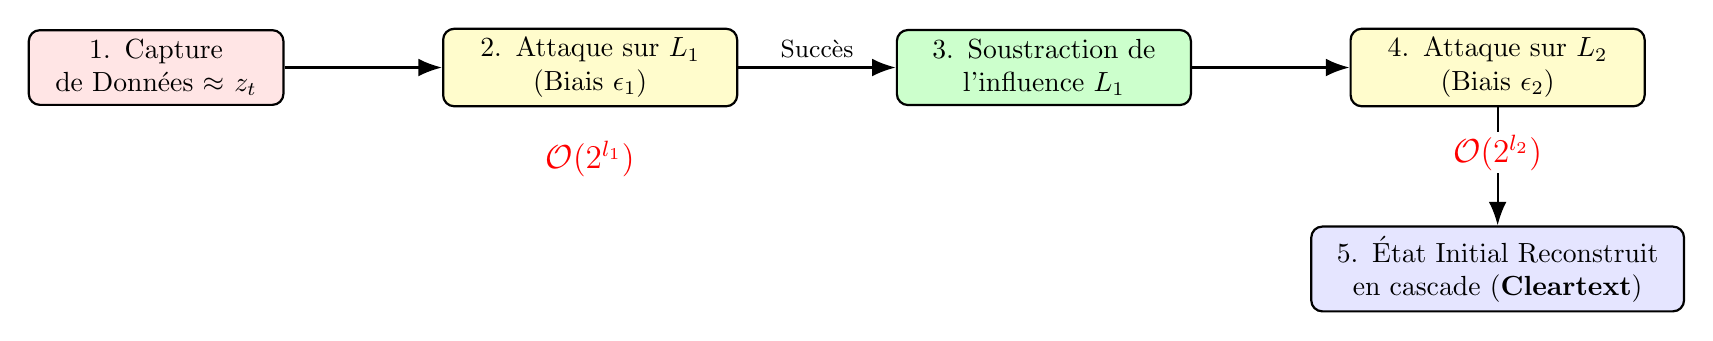
\begin{tikzpicture}[auto, thick, node distance=1.5cm and 2cm]
        % Nodes
        \node[draw, rounded corners, fill=red!10, text width=3cm, align=center] (capture) {1. Capture\\de Données $\approx z_t$};
        \node[draw, rounded corners, fill=yellow!20, text width=3.5cm, align=center, right=of capture] (attack1) {2. Attaque sur $L_1$\\ (Biais $\epsilon_1$)};
        \node[draw, rounded corners, fill=green!20, text width=3.5cm, align=center, right=of attack1] (remove1) {3. Soustraction de\\ l'influence $L_1$};
        \node[draw, rounded corners, fill=yellow!20, text width=3.5cm, align=center, right=of remove1] (attack2) {4. Attaque sur $L_2$\\ (Biais $\epsilon_2$)};
        
        \node[draw, rounded corners, fill=blue!10, text width=4.5cm, align=center, below=1.5cm of attack2] (finish) {5. État Initial Reconstruit\\ en cascade (\textbf{Cleartext})};

        % Arrows
        \draw[-{Latex[length=3mm]}] (capture) -- (attack1);
        \draw[-{Latex[length=3mm]}] (attack1) -- node[above, font=\small] {Succès} (remove1);
        \draw[-{Latex[length=3mm]}] (remove1) -- (attack2);
        \draw[-{Latex[length=3mm]}] (attack2) -- (finish);

        % Annotations Complexities
        \node[below=0.3cm of attack1, text=red, font=\large] {$\mathcal{O}(2^{l_1})$};
        \node[below=0.3cm of attack2, fill=white, inner sep=1pt, text=red, font=\large] {$\mathcal{O}(2^{l_2})$};
    \end{tikzpicture}
    }
    \end{center}

    \vspace{0.3cm}
    \textbf{Le processus itératif de l'attaque NSA} :
    \begin{enumerate}
        \item Capter le chiffré cible, et y associer du "Plaintext-Probable" (mot connu, salutation diplomatique, entête télex).
        \item Simuler le registre $L_1$ pour toutes ses clés partielles ($2^{l_1}$ états).
        \item Conserver la clé de $L_1$ qui valide la plus haute corrélation avec le bruit.
        \item Affaiblir mathématiquement le résidu et continuer sur les registres suivants.
    \end{enumerate}

    \note{
        Voici schématiquement comment je modélise l'attaque en cascade appliquée concrètement sur les flux télégraphiques de la NSA.
        
        A l'étape 1, j'intercepte le flux. En modélisant le "plaintext probable" (comme on l'étudie classiquement, de l'en-tête diplomatique redondante du format "To Mr Ambassador"), je réalise le calcul du XOR exclusif.
        
        Une fois cette information de base captée, à vide, mon supercalculateur compare l'état du tout premier registre simulé aux bits capturés, assisté par l'analyse algorithmique de ce fameux "bruit" statistique. Quand une clé partielle concorde, je l'isole par le fort pic de corrélation (ici en étape 2). 
        
        Je soustrait ensuite "l'influence" (étape 3) de ce premier module cassé, purifie les calculs suivants, et relance simplement cette cascade pour les registres L2 puis L3 ! Le système s'effondre de l'intérieur, de registre en registre. Le chiffrement est cassé !
    }
\end{frame}

% ==============================================================================
% 6. LA CHUTE DE L'EMPIRE CRYPTO AG (HANS BÜHLER)
% ==============================================================================
\section{La Chute d'Operation Rubicon}

\begin{frame}{1992 : La Faille Humaine (L'Affaire Hans Bühler)}
    \begin{columns}
        \column{0.6\textwidth}
        \textbf{L'Arrestation en Iran}
        \begin{itemize}
            \item Hans Bühler, ingénieur commercial star de Crypto AG, est brusquement arrêté à Téhéran en 1992.
            \item Le gouvernement Iranien suspecte l'équipement d'être compromis suite à des fuites liées à des assassinats politiques.
        \end{itemize}

        \vspace{0.3cm}
        \textbf{L'Opération Démasquée}
        \begin{itemize}
            \item La CIA et le BND refusent d'intervenir pour protéger la couverture.
            \item Crypto AG finit par payer une étrange rançon/caution de 1\text{M} \$ à l'Iran, puis licencie Bühler.
            \item L'attention médiatique fait s'écrouler le mythe inviolable de la "neutralité suisse".
        \end{itemize}

        \column{0.4\textwidth}
        \begin{center}
            \begin{alertblock}{La Couverture Parfaite}
                Bühler, comme l'immense majorité des ingénieurs suisses de Crypto AG, ignorait totalement la manipulation des schémas d'immunité des LFSR par Minerva !
            \end{alertblock}
        \end{center}
    \end{columns}

    \note{
        Mais alors, si le système était mathématiquement pur en surface, comment l'empire secret Rubicon s'est-il finalement effondré ?

        Ironiquement pour nous analystes d'algorithmes, ce n'est pas un audit cryptographique qui a révélé la faille, mais une grossière erreur humaine ! En 1992, Hans Bühler, un des vendeurs phares de Crypto AG qui vendait ces machines au Moyen-Orient, est brusquement emprisonné par l'Iran. Les iraniens s'étaient rendus compte que l'Ouest anticipait de manière trop miraculeuse leurs frappes terroristes et politiques, et ont logiquement pointé du doigt l'intégrité de ces machines suisses qu'on leur avait lourdement facturées.

        Bühler, qui n'était pas au courant de la fraude, reste emprisonné neuf mois. La CIA a catégoriquement refusé de lever le petit doigt pour ne pas "griller" la couverture technologique. Dès sa libération sous caution, ce traitement injuste le poussera à alerter la presse germanique. De fil en aiguille, les journalistes d'investigation trouveront la relation cachée entre l'usine de Zoug et le BND à Munich. Le secret industriel du siècle venait de s'éteindre.
    }
\end{frame}

\begin{frame}{2020 : La Déclassification et le Washington Post}
    \begin{columns}
        \column{0.55\textwidth}
        \textbf{Le Secret Révélé (\#CRYPTOLEAKS)}
        \begin{itemize}
            \item En Février 2020, une enquête conjointe du \textit{Washington Post} (USA), de la \textit{ZDF} (ALL) et de \textit{SRF} (SUI) dévoile l'entièreté du scandale.
            \item Ils publient des documents de la CIA déclassifiés, prouvant que de 1970 à 1993, la quasi-totalité des communications sécurisées mondiales étaient lues par la NSA.
        \end{itemize}

        \vspace{0.3cm}
        \textbf{Le Coup de Maître}
        \begin{itemize}
            \item Un rapport interne de la CIA décrit l'opération Rubicon comme "Le coup de maître du renseignement du siècle".
        \end{itemize}

        \column{0.45\textwidth}
        \begin{center}
            \includegraphics[height=3.5cm]{images/hagelin.jpg}\\
            \vspace{0.1cm}
            \small \textit{Machine classique Hagelin réputée inviolable.}
        \end{center}
    \end{columns}

    \note{
        Pour conclure définitivement sur ce pan d'histoire, comment a-t-on la certitude absolue de la véracité de cette incroyable opération ?

        En Février 2020 (il y a à peine quelques années), une enquête coup de poing mondiale entre le Washington Post, la télévision allemande et la télévision suisse ont publié ce qu'ils appellent les "Cryptoleaks". Des documents top-secrets de la CIA ont été déclassifiés, et ont formellement prouvé que de 1970 jusqu'à la fin de la guerre froide, ce duo contrôlait plus de 40\% des flux mondiaux cryptés.

        Un rapport interne de l'agence va même jusqu'à qualifier Rubicon de "coup de maître du renseignement du siècle". La société Crypto AG a finalement été liquidée en 2018. Des décennies de communications ultra-secrètes ont été aspirées silencieusement, le tout à cause d'un décalage mathématique subtil sur un polynome de LFSR.
    }
\end{frame}

% ==============================================================================
% 6. REFERENCES (SECOND TO LAST SLIDE)
% ==============================================================================
\section{Références}

\begin{frame}{Références Bibliographiques}
    \begin{itemize}
        \item \textbf{Support de Cours Fondamental :}
        \begin{itemize}
            \item G. Castagnos, \textit{Cours de Cryptologie 2025-2026}, Univ. Bordeaux.
            \item \textit{Chapitre II : Chiffrement par flot, suites pseudo-aléatoires, LFSR et propriétés d'immunité.}
            \item Support formel pour la modélisation mathématique du Berlekamp-Massey et de la complexité algorithmique.
        \end{itemize}

        \vspace{0.4cm}
        \item \textbf{Aspects Géopolitiques \& Sources Opérationnelles :}
        \begin{itemize}
            \item \textit{The intelligence coup of the century} (Operation Rubicon). Greg Miller, Washington Post, 2020.
            \item \textit{"The Swiss Cheese of Cryptography: Historical hardware and modern analysis"}, Thomas Pornin, SSTIC (\textit{Symposium sur la sécurité des technologies de l'information}).
            \item Analyse Reverse-Engineering des HC-7000, J. Gressel \& Chaos Computer Club (CCC), Projet \textit{\#CRYPTOLEAKS}, Leipzig (2020).
        \end{itemize}
    \end{itemize}
    \note{
        Afin de formaliser au mieux ce cours et de rigoureusement valider mes calculs et asymétries de modélisation mathématique du Berlekamp-Massey, je me suis basé sur notre Chapitre 2 du Master. C'est véritablement grâce au "Cours de Cryptologie" de Monsieur Guilhem Castagnos que j'ai pu illustrer pourquoi un algorithme d'apparence sûre pour le grand public s'avérait tragiquement manipulable.
        
        Sur l'aspect du gigantesque scandale "Opération Rubicon", les documents formels déclassifiés par le Washington Post en 2020 ont guidé mes bases. L'exploration de la "faille Minerva", quant-à-elle, trouve ses repères visuels par l'impressionnant travail de reverse-engineering dévoilé ici-même à Leipzig en 2020 par the Chaos Computer Club. 
    }
\end{frame}

% ==============================================================================
% 7. CONCLUSION
% ==============================================================================
\section{Conclusion}

\begin{frame}
    \centering
    \Huge \textbf{Questions ?}

    \vspace{1cm}
    \normalsize
    \textit{"Trust, but Verify."}\\
    \vspace{0.2cm}
    \small -- \textbf{Ronald Reagan} (Proverbe des sommets sur le nucléaire, Guerre Froide)
    
    \vspace{0.5cm}
    \normalsize
    \textit{Ou plutôt aujourd'hui : "Trust no one, and Open-Source everything."}

    \note{
        J'arrivais donc à l'irréfutable conclusion que l'Opération Rubicon marque la fin définitive du concept dangereux de "Security by Obscurity".
        
        L'histoire vient ici nous démontrer rudement que confier le secret de communications étatiques à un matériel propriétaire et exclusif non certifié de façon ouverte – même Suisse ! – ouvre la porte à des failles à l'échelle mondiale.
        
        Je suis intimement convaincu qu'en tant que professionnels de la SSI de demain, seule l'ouverture public ("Open-Source algorithms" du type AES ou standards NIST certifiés), associée au contrôle d'audit de sécurité des communautés mathématiques, pourra empêcher ce type de vulnérabilités ! "Trust no one".
        
        Je vous remercie vivement pour m'avoir écouté pendant ces 15 minutes. N'hésitez-pas si vous avez des questions sur l'algorithmique LFSR, la notion de Corrélation ou même sur cette incroyable affaire d'espionnage, je serai ravi d'y répondre. 
    }
\end{frame}

\end{document}